\begin{figure}
  \centering
  \begin{tikzpicture}
    \node at (-3,0) {
      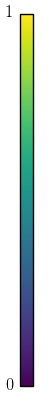
\includegraphics[height=5.5cm]{experiments/2d/vae_occ_sdf_aml/colorbar_0}
    };
    
    \node at (0, 0){
      \includegraphics[width=5cm]{experiments/2d/vae_occ_sdf_aml/easy_5_long/results_0}
    };
    \node at (0, -5.5){
      \includegraphics[width=5cm]{experiments/2d/vae_occ_sdf_aml/hard_5_long/results_0}
    };
    \node at (0, -9.5){
      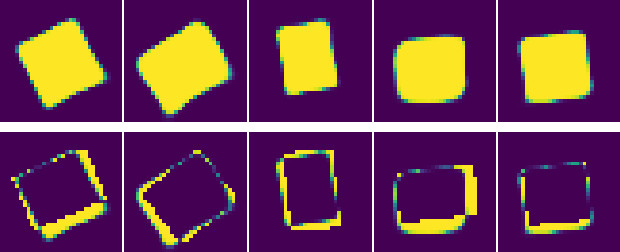
\includegraphics[height=2cm]{experiments/2d/vae_occ_sdf_aml/hard_5_long_statistics/results_0_only}
    };
    
    \draw[-,dashed] (2.75, -10.5) -- (2.75,3);
    
    \node at (5.5, 0){
      \includegraphics[width=5cm]{experiments/2d/vae_occ_sdf_aml/easy_5_long/results_1}
    };
    \node at (5.5, -5.5){
      \includegraphics[width=5cm]{experiments/2d/vae_occ_sdf_aml/hard_5_long/results_1}
    };
    \node at (5.5, -9.5){
      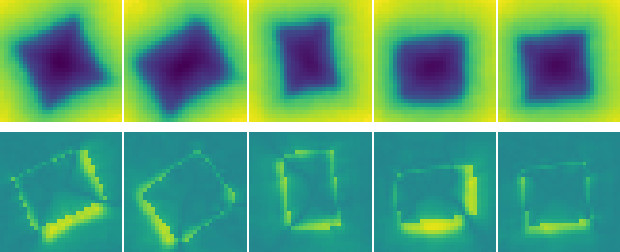
\includegraphics[width=5cm]{experiments/2d/vae_occ_sdf_aml/hard_5_long_statistics/results_1_only}
    };
    
    \node at (8.5,0) {
      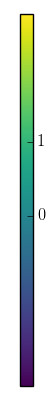
\includegraphics[height=5.5cm]{experiments/2d/vae_occ_sdf_aml/colorbar_1}
    };
    
    %\node[rotate=90] at (-3,0) {\easy};
    \node[rotate=90] at (-3,-5.5) {\hard};
    \draw[-,dashed] (-3,-2.75) -- (8.5,-2.75);
   
    \node[rotate=90] at (-3,-9.5) {\hard *};
    \draw[-,dashed] (-3,-8.25) -- (8.5,-8.25);
   
    \node at (0, 3) {occupancy};
    \node at (5.5, 3) {signed distance function};
  \end{tikzpicture}
  \vskip 6px
  
  % TODO short caption
  \caption{Qualitative results for \AML predicting both modalities, \ie
  occupancy and signed distance functions. We show results for both the \easy and
  the \hard case. For the
  easy case, we show the observed points, the corresponding free space and the
  target shape; followed by the prediction and the corresponding error.
  For the hard case we follow the same procedure, however, we also show results
  using the weighted loss.}
  \label{fig:experiments-2d-sdf-aml-qual}
\end{figure}
